\chapter{La situation de référence}
\label{ch:reference}

Toutes les expériences de ce rapport comparent un avenir « avec mesure » à un avenir « sans mesure ». Ce second
avenir, la \emph{trajectoire de référence à politique inchangée}, est construit en trois temps (fichier
\code{src/m8\_reference.py}) :
\begin{enumerate}
\item \textbf{2023-2025} : le modèle reproduit les comptes observés (Insee, comptes annuels publiés en mai 2026) grâce à
des termes de calage ajoutés aux équations ;
\item \textbf{2026-2031} : la croissance, le chômage et l'inflation suivent les projections du FMI (octobre 2026) ; les
finances publiques sont calculées par le modèle, sans les mesures de redressement que le FMI suppose ;
\item \textbf{après 2031} : productivité par tête +0,7~\% par an et chômage convergeant vers 7~\% (hypothèses centrales
du COR), taux de l'OAT maintenu à 4,89~\%, consommation publique en volume +1,3~\% par an.
\end{enumerate}
Ce n'est pas une prévision : c'est un point de comparaison commun, qui contient ses propres incertitudes. En
particulier, une trajectoire « sans aucune mesure nouvelle pendant vingt ans » n'est pas réaliste ; elle sert à mesurer
l'ampleur des problèmes à résoudre.

\section{Le modèle face aux statistiques observées}

Le tableau~\ref{tab:reference} confronte les grandeurs du modèle aux statistiques publiées. Pour les comptes
nationaux 2023-2025, la concordance est forte \emph{par construction} (calage) : elle vérifie la cohérence comptable,
pas la capacité prédictive. Pour les indicateurs qui ne sont pas calés (niveau de vie, pauvreté, solde extérieur,
pouvoir d'achat), les écarts sont importants et doivent être lus comme des limites du modèle.

\begin{small}
\begin{longtable}{@{}p{4.6cm}rrp{5.2cm}@{}}
\caption{Situation de référence : modèle et statistiques observées (2025 sauf mention).}\label{tab:reference}\\
\toprule
Indicateur & Modèle & Observé & Source de l'observé ; commentaire \\
\midrule\endfirsthead
\toprule Indicateur & Modèle & Observé & Source ; commentaire \\ \midrule\endhead
\bottomrule\endfoot
\multicolumn{4}{@{}l}{\textit{Activité}} \\
PIB en valeur (Md€) & 2\,991 & 2\,991,1 & Insee, comptes de la Nation 2025 (juin 2026) ; calé \\
Croissance du PIB en volume (\%) & 0,81 & 0,8 & idem ; 2024 : 1,51 contre 1,5 \\
PIB par habitant (€) & 43\,370 & 43\,370 & PIB / population moyenne (M1 : 68,97 M) \\
Productivité par tête (\%) & +0,66 & -- & PIB en volume / emploi ; non publié directement \\
Emploi (millions) & 30,64 & calé & Comptes nationaux (Eurostat) \\
Chômage BIT (\%) & 7,44 & 7,7 & Insee, enquête Emploi, France hors Mayotte ; le modèle utilise la série France métropolitaine (moyenne 2025 : 7,5) \\
\multicolumn{4}{@{}l}{\textit{Revenus et demande des ménages}} \\
Salaire moyen par tête (\%) & +2,1 & -- & calé sur les comptes de branche \\
Revenu disponible brut (Md€) & 1\,906 & -- & calé en 2023-2025 \\
Pouvoir d'achat du RDB (\%) & +1,5 & $-$0,7 par UC & Insee Première 2105 ; \textbf{écart} : chute des dividendes reçus en 2025 non captée \\
Consommation en volume (\%) & +0,61 & +0,4 & Insee Première 2105 \\
Taux d'épargne (\% du RDB) & 17,86 & 17,8 & Insee, comptes trimestriels (T1 2026) \\
Investissement en volume (\%) & +0,48 & +0,5 & Insee Première 2105 \\
\multicolumn{4}{@{}l}{\textit{Niveau de vie (microsimulation, revenus 2024)}} \\
Niveau de vie médian (€/UC/an) & 22\,179 & 26\,740 & Insee Première 2117 (2024) ; \textbf{non comparable} : revenus non imposables omis \\
Taux de pauvreté à 60~\% (\%) & 17,3 & 15,4 & idem ; seuil 1\,337~€/mois \\
Indice de Gini & 0,349 & 0,30 & idem ; inégalités surestimées \\
Rapport interdécile D9/D1 & 4,10 & 3,5 & idem \\
\multicolumn{4}{@{}l}{\textit{Échanges extérieurs et énergie}} \\
Solde courant (\% du PIB) & +2,9 & $-$0,4 & Banque de France, balance des paiements 2025 ($-$11,6\md) ; \textbf{niveau non fiable} \\
Solde des biens (Md€) & -- & $-$60,1 & idem ; dont énergie $-$42,4 \\
Indépendance énergétique (\%) & -- & 62,7 & SDES, bilan provisoire 2025 ; non représentée en quantités \\
\multicolumn{4}{@{}l}{\textit{Finances publiques}} \\
Dépenses publiques (\% du PIB) & 57,3 & 57,2 & Insee, comptes des APU 2025 (mars 2026) ; calé \\
Recettes publiques (\% du PIB) & 52,2 & 52,1 & idem \\
Solde public (\% du PIB) & $-$5,07 & $-$5,1 & idem \\
Dette publique (\% du PIB) & 115,7 & 115,6 & idem (115,7 dans la version de mai 2026) \\
Charge d'intérêts (\% du PIB) & 2,47 & -- & calé sur les comptes \\
Prestations sociales en espèces (Md€) & 555 & calé & comptes nationaux (D62) \\
Pensions de droit direct (\% du PIB) & 13,5 & -- & M9 \\
\end{longtable}
\end{small}

\begin{encadre}{Encadré 4.1 — Pourquoi le niveau de vie du modèle diffère de celui de l'Insee}
L'Insee mesure le niveau de vie à partir de l'enquête Revenus fiscaux et sociaux, qui apparie les déclarations de
revenus et les prestations effectivement versées. Le modèle reconstitue les revenus d'un échantillon de ménages réels
à partir de distributions publiées : il ne voit ni les revenus exonérés (une partie des revenus du patrimoine, les
heures supplémentaires défiscalisées réintégrées imparfaitement), ni les prestations non simulées (allocations de
rentrée, prestations d'invalidité…). Le niveau de vie médian est donc trop bas de 17~\% et la dispersion trop forte.
En revanche, quand on compare deux législations sur \emph{le même échantillon}, ces erreurs se compensent en grande
partie : c'est pourquoi le rapport n'utilise la microsimulation que pour des \textbf{variations} (effet d'une mesure sur
le taux de pauvreté au seuil fixe, variation de l'indice de Gini, gains et pertes par décile).
\end{encadre}

\section{La trajectoire de référence jusqu'en 2047}

\begin{figure}[htbp]
\centering
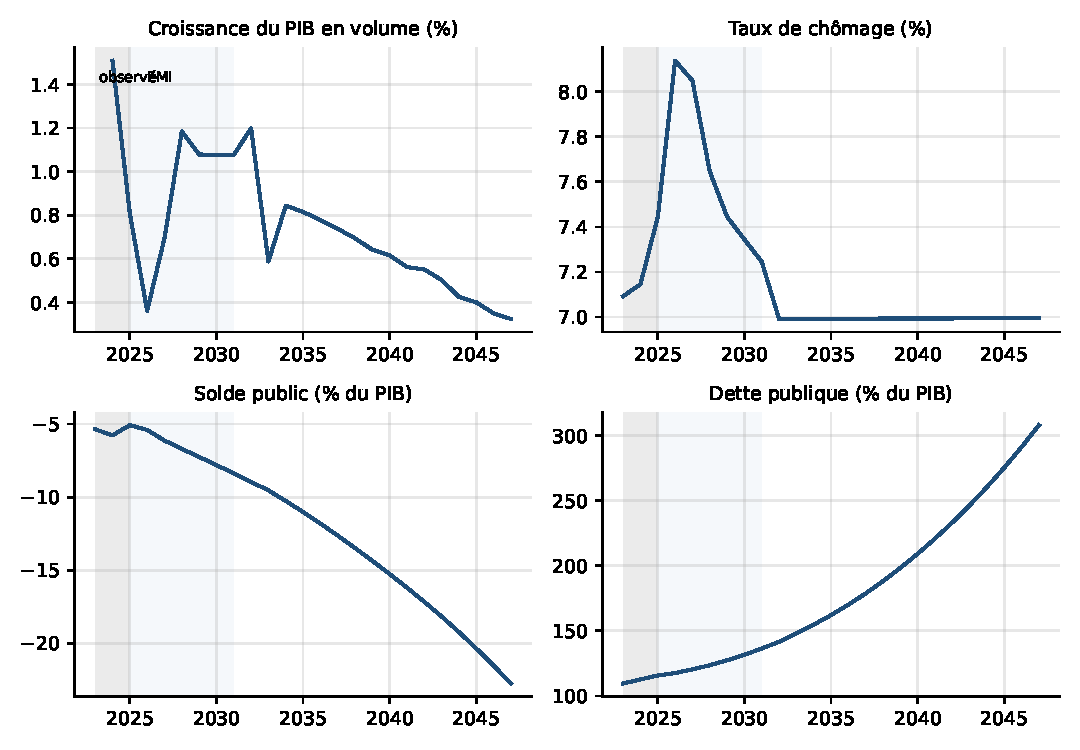
\includegraphics[width=\linewidth]{reference.pdf}
\caption{Trajectoire de référence à politique inchangée. Zone grise : années observées et reproduites ; zone bleutée :
projections calées sur le FMI ; au-delà, hypothèses du COR et du modèle.}
\label{fig:reference}
\end{figure}

\begin{table}[htbp]
\centering\small
\caption{Principaux indicateurs de la trajectoire de référence.}
\label{tab:refproj}
\begin{tabular}{@{}lrrrrrr@{}}
\toprule
 & 2025 & 2026 & 2030 & 2032 & 2037 & 2047 \\
\midrule
Croissance du PIB (\%) & 0,81 & 0,36 & 1,08 & 1,20 & 0,74 & 0,32 \\
Chômage (\%, métropole) & 7,44 & 8,14 & 7,34 & 6,99 & 6,99 & 7,00 \\
Inflation (\%) & 0,83 & 2,37 & 1,88 & 1,78 & 1,78 & 1,76 \\
Taux d'épargne (\%) & 17,9 & 17,6 & 16,0 & 15,5 & 15,5 & 15,5 \\
Solde public (\% du PIB) & $-$5,1 & $-$5,4 & $-$7,8 & $-$9,0 & $-$12,6 & $-$22,8 \\
Dette publique (\% du PIB) & 115,7 & 117,6 & 131,5 & 141,6 & 178,8 & 308,2 \\
Charge d'intérêts (\% du PIB) & 2,5 & 2,9 & 4,4 & 5,1 & 7,2 & 13,6 \\
Pensions de droit direct (\% du PIB) & 13,5 & 13,3 & 14,0 & 14,2 & 14,7 & 15,7 \\
Industrie manufacturière (\% du PIB) & 9,6 & 9,5 & 9,0 & 8,7 & 8,4 & 9,2 \\
Emploi (millions) & 30,64 & 30,50 & 31,23 & 31,53 & 31,67 & 31,25 \\
Population active (millions) & 33,10 & 33,21 & 33,71 & 33,90 & 34,05 & 33,60 \\
Plus de 65 ans / 20-64 ans & 0,39 & 0,40 & 0,43 & -- & 0,47 & 0,51 \\
\bottomrule
\end{tabular}
\end{table}

\paragraph{Lecture.} Quatre dynamiques dominent la référence.
\begin{enumerate}
\item \textbf{Une croissance faible et déclinante} : 1,1 à 1,2~\% jusqu'en 2032, puis moins de 0,8~\% par an, puis
0,3~\% en fin de période. Elle résulte de la productivité supposée (+0,7~\% par tête) et du plafonnement puis du recul
de la population active à partir du milieu des années 2030 (vieillissement, fécondité de 1,45). La croissance est donc
d'abord une question de \emph{productivité} et de \emph{nombre d'actifs}.
\item \textbf{Une dérive des finances publiques} : sans mesure, le déficit passe de 5,1 à 9~\% du PIB en 2032. Les
causes, par ordre d'importance : la charge d'intérêts (de 2,5 à 5,1 points de PIB, car la dette émise à 1-2~\% est
progressivement refinancée à près de 5~\%), la hausse des pensions avec le vieillissement, et une dépense publique en
volume qui croît plus vite que l'activité (1,3~\% par an contre 1,1~\%). Au-delà, l'« effet boule de neige » rend la
trajectoire explosive. Le FMI, qui suppose un redressement non encore voté, projette un solde de $-$3,9~\% et une dette
de 124~\% en 2031 : l'écart, environ 4 points de PIB, mesure l'effort que ce redressement représenterait.
\item \textbf{Un vieillissement qui pèse sur la protection sociale} : 0,39 personne de 65 ans ou plus pour une personne
de 20 à 64 ans en 2025, 0,47 en 2037, 0,51 en 2047 ; les pensions passent de 13,5 à 15,7~\% du PIB.
\item \textbf{Une désindustrialisation tendancielle} : la part de l'industrie manufacturière baisse jusqu'à 8,4~\% en
2037. La remontée de la fin de période est un artefact (prix relatifs de 2022 non chaînés) qu'il ne faut pas
interpréter.
\end{enumerate}

\begin{limites}[Fiabilité de la référence]
Les comptes 2023-2025 sont reproduits \fiab{robuste}. Les projections 2026-2031 reprennent celles du FMI pour la
croissance, le chômage et l'inflation \fiab{conventionnel}. Les finances publiques sont calculées par le modèle : leur
dérive est \fiab{plutôt robuste} dans son sens (taux d'intérêt et démographie), \fiab{fragile} dans son ampleur au-delà
de 2035 (hypothèse de taux constant à 4,89~\%, absence de toute réaction de politique économique). Le solde extérieur
de la référence se dégrade continûment (de +2,9 à $-$7,7~\% du PIB) sous l'effet de la tendance de pénétration des
importations estimée sur 1997-2019 : \fiab{non établi}.
\end{limites}
